\section{Addition, Subtraction, and Multiplication}
Algebra is ultimately about applying some procedure, or sequence of procedures, to numbers, and asking which numbers yield some desired result. To this end, we need to conceptualize numbers more dynamically than just as a way of counting objects. In the following table we present a way to conceptualize numbers as positions on a line, and the basic operations as movements.  


\begin{center}

\begin{table}
\begin{tabular}{|p{2in} c p{1.5in}|}
\hline\hline \it{Positions and Sizes} & & \it{Numbers}\\
\hline Location on a Line & $\longrightarrow$ & Number \\&&\\
Center of the Line & $\longrightarrow$ & $0$ \\&&\\
Position to the Right of Center & $\longrightarrow$ & Positive Number \\&&\\
Position to the Left of Center & $\longrightarrow$ & Negative Number \\&&\\
One Step to the Right & $\longrightarrow$ & 1 \\&&\\
Given a position $a$, the position that is the same distance from the center on  the opposite side & $\longrightarrow$ & $-a$\\&&\\ 
Starting from   $a$, and moving  the same distance that $b$ is from the center & $\longrightarrow$ & $a+b$\\&&\\
Starting from $a$, and moving the distance in the opposite direction that $b$ is from the center & $\longrightarrow$ & $a-b$\\&&\\
When $a$ and $b$ are positive, the number whose size relative to $b$ is the same as the size of $a$ relative to $1$ & $\longrightarrow$ & $ab$\\&&\\
$a$ is to the right of $b$ & $\longrightarrow$ & $b<a$\\&&\\
$a$ is to the left of $b$ & $\longrightarrow$ & $a<b$\\&&\\
\hline
\end{tabular} 
\caption{Addition, Subtraction, and Multiplication as Motions on the Line} \label{tab:a}
\end{table}
\end{center}


In order to understand what's going on here, it will be useful to draw  pictures. This is a picture of the real number line that you've probably seen before:\\
\vspace{.2in}
\begin{figure}[h]
\centering
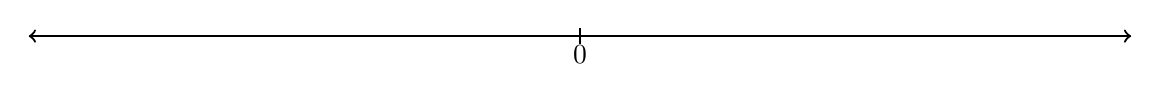
\begin{tikzpicture}
\draw[thick] [->] (0,0) -- (7,0);
\draw[thick] [<-] (-7,0) -- (0,0);
\draw (0,-.1) -- (0,.1);
\node[align=center,below] at (0,0){0};
\end{tikzpicture}
\caption{The basic number line.}
\end{figure}

This picture does not show us much, so let's show one with some generic numbers $a$ and $b$, where both $a$ and $b$ are positive with $b>a$.
\vspace{.2in}
\begin{figure}[h]
\centering
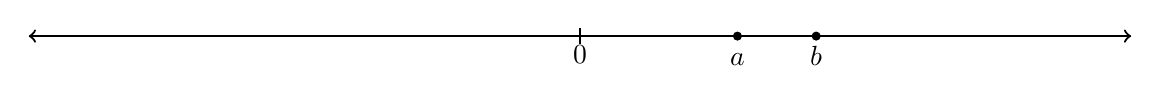
\begin{tikzpicture}
\draw[thick] [->] (0,0) -- (7,0);
\draw[thick] [<-] (-7,0) -- (0,0);
\draw (0,-.1) -- (0,.1);
\node[align=center,below] at (0,0){$0$};
\node[align=center,below] at (2,-.1){$a$};\draw[fill](2,0)circle[radius=.05];
\node[align=center,below] at (3,0){$b$};\draw[fill](3,0)circle[radius=.05];
\end{tikzpicture}
\caption{A number line with two  positive numbers labeled.}
\end{figure}

To represent $a+b$ and $a-b$ geometrically, we first measure out the distance $b$ is to the right of zero, then move that far to the right of $a$ for $a+b$ and move that distance to the left of $a$ for $a-b$.

\vspace{.2in} 
\begin{figure}[h]
\centering
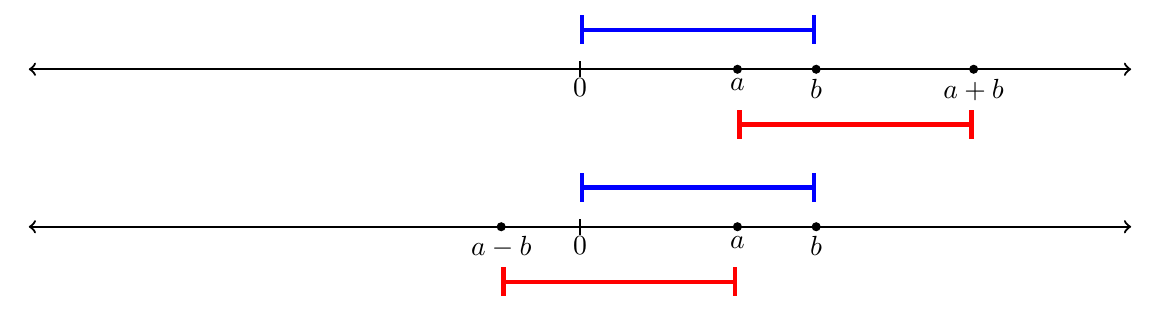
\begin{tikzpicture}
\draw[ultra thick,blue][|-|] (0,2.5) -- (3,2.5);
\draw[ultra thick,red][|-|] (2,1.3) -- (5,1.3);
%\draw[ultra thick,red][|-|] (-1,-.7) -- (2,-.7);
\draw[thick] [->] (0,2) -- (7,2);
\draw[thick] [<-] (-7,2) -- (0,2);
\draw (0,1.9) -- (0,2.1);
\node[align=center,below] at (0,2){$0$};
\node[align=center,below] at (2,2){$a$};\draw[fill](2,2)circle[radius=.05];
\node[align=center,below] at (3,2){$b$};\draw[fill](3,2)circle[radius=.05];
\node[align=center,below] at (5,2){$a+b$};\draw[fill](5,2)circle[radius=.05];
%\node[align=center,below] at (-1,0){$a-b$};\draw[fill](-1,0)circle[radius=.05];

\draw[ultra thick,blue][|-|] (0,.5) -- (3,.5);
%\draw[ultra thick,red][|-|] (2,-.7) -- (5,-.7);
\draw[ultra thick,red][|-|] (-1,-.7) -- (2,-.7);
\draw[thick] [->] (0,0) -- (7,0);
\draw[thick] [<-] (-7,0) -- (0,0);
\draw (0,-.1) -- (0,.1);
\node[align=center,below] at (0,0){$0$};
\node[align=center,below] at (2,0){$a$};\draw[fill](2,0)circle[radius=.05];
\node[align=center,below] at (3,0){$b$};\draw[fill](3,0)circle[radius=.05];
%\node[align=center,below] at (5,0){$a+b$};\draw[fill](5,0)circle[radius=.05];
\node[align=center,below] at (-1,0){$a-b$};\draw[fill](-1,0)circle[radius=.05];
\end{tikzpicture}
\caption{Addition and subtraction of positive numbers.}
\label{fig:addsubt1}
\end{figure} 


In Figure \ref{fig:addsubt1}, since $b>a$ we end up to the left of zero when we subtract $b$ from $a$. This should make sense; if you take away more than you started out with, you end up with a deficit.

\par

\begin{question} \begin{enumerate}
   \item[a.] With $a$ and $b$ in the same positions as in Figure \ref{fig:addsubt1}, draw $b+a$.   What do you notice about $a+b$ in relation to $b+a$? \item[b.] Now draw $b-a$.  Is the same relationship true for $a-b$ and $b-a$?  \end{enumerate}
\end{question}
\par
\begin{question} Draw a number line with numbers $a$ and $b$ on it, but this time make $a$ positive and $b$ negative. Is $a+b$ to the right or left of $a$? Explain.  
\end{question}
\par
\begin{question} Explain why $0+a = a$ for any number $a$.
\end{question}
\par

One of the important ideas in algebra is that of {\bf inverse operations}. We can see this idea by looking at subtraction. Observe that if $a$ and $b$ are numbers, then $a+b-b = a$. This may seem obvious, especially if you draw it on the number line. However, the concept is very important; \itshape the inverse of adding  $b$ to $a$ is subtracting $b$. \upshape We may say that subtracting ``undoes'' addition or that when you add and subtract the same quantity they ``cancel each other''. 


\par 

Multiplication is more difficult to visualize  geometrically, but the fundamental idea is that of  stretching, with $1$ being a basic unit of measurement. Let's start with $b$ being any positive number and $a=1.5$.  We see that $1$ fits into $a$ exactly  $1.5$ times.  Since $ab$ must have the same size relative to $b$ as $a$ does to $1$, $b$ must fit into $ab$ exactly $1.5$ times. Think of this as stretching $b$ by a factor of $a$ when $a>1$.\\

\vspace{.2in} 
\begin{figure}[h]
\centering
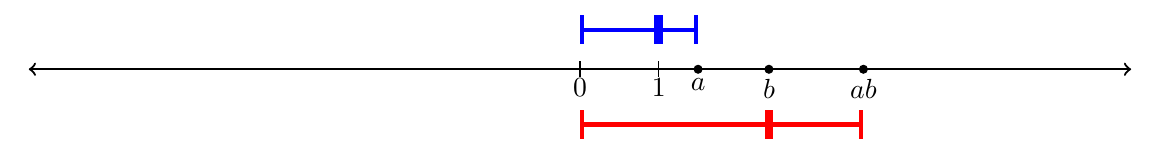
\begin{tikzpicture}
\draw[ultra thick,blue][|-|] (0,.5) -- (1,.5);
\draw[ultra thick,blue][|-|] (1,.5) -- (1.5,.5);
\draw[ultra thick,red][|-|] (0,-.7) -- (2.4,-.7);
\draw[ultra thick,red][|-|] (2.4,-.7) -- (3.6,-.7);
\draw[thick] [->] (0,0) -- (7,0);
\draw[thick] [<-] (-7,0) -- (0,0);
\node[align=center,below] at (0,0){$0$};\draw (0,-.1) -- (0,.1);
\node[align=center,below] at (1,0){$1$};\draw (1,-.1) -- (1,.1);
\node[align=center,below] at (2.4,0){$b$};\draw[fill](2.4,0)circle[radius=.05];
\node[align=center,below] at (1.5,0){$a$};\draw[fill](1.5,0)circle[radius=.05];
\node[align=center,below] at (3.6,0){$ab$};\draw[fill](3.6,0)circle[radius=.05];
\end{tikzpicture}
\caption{The same number of copies of $b$ are in $ab$ as copies of $1$ are in $a$.}
\label{fig:mult1}
\end{figure}


If $a$ is smaller than $1$, for example $a = 0.75$, then you don't get a whole copy of $1$ in $a$, you only have $75\%$ of one. This means you will only get $75\%$ of a copy of $b$ in $ab$. In the case when $a<1$, we think of $ab$ as a squeeze of $b$ by a factor of $a$.\\

\vspace{.2in}
\begin{figure}[h]
\centering
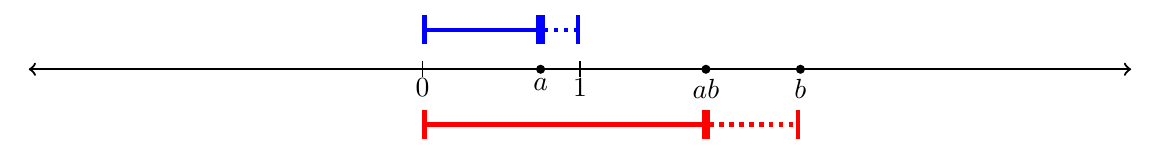
\begin{tikzpicture}
\draw[ultra thick,blue][|-|] (-2,.5) -- (-.5,.5);
\draw[ultra thick,dotted,blue][|-|] (-.5,.5) -- (0,.5);
\draw[ultra thick,red][|-|] (-2,-.7) -- (1.6,-.7);
\draw[ultra thick,dotted,red][|-|] (1.6,-.7) -- (2.8,-.7);
\draw[thick] [->] (0,0) -- (7,0);
\draw[thick] [<-] (-7,0) -- (0,0);
\node[align=center,below] at (-2,0){$0$};\draw (-2,-.1) -- (-2,.1);
\node[align=center,below] at (0,0){$1$};\draw (0,-.1) -- (0,.1);
\node[align=center,below] at (2.8,0){$b$};\draw[fill](2.8,0)circle[radius=.05];
\node[align=center,below] at (-.5,0){$a$};\draw[fill](-.5,0)circle[radius=.05];
\node[align=center,below] at (1.6,0){$ab$};\draw[fill](1.6,0)circle[radius=.05];
\end{tikzpicture}
\caption{If $a<1$, then $ab$ is the same percentage of $b$ as $a$ is of $1$.}
\label{fig:mult2}
\end{figure} 

\pagebreak

An important case happens when one of the two numbers is a whole number (an integer). If $n$ is a positive integer, then $1$ fits into $n$ exactly $n$ times. Hence, if $b$ is positive, $b$ will fit into $nb$ exactly $n$ times. Let's view this on the number line with $n=5$:

\vspace{.2in} 
\begin{figure}[h]
\centering
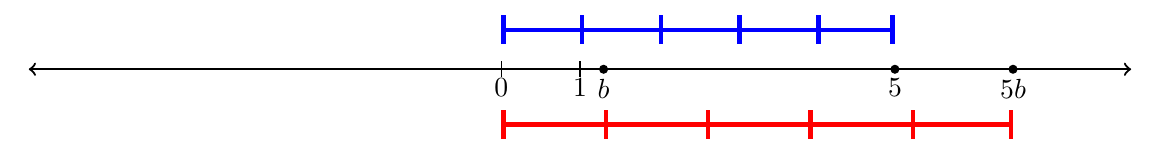
\begin{tikzpicture}
\draw[ultra thick,blue][|-] (-1,.5) -- (0,.5);
\draw[ultra thick,blue][|-] (0,.5) -- (1,.5);
\draw[ultra thick,blue][|-] (1,.5) -- (2,.5);
\draw[ultra thick,blue][|-] (2,.5) -- (3,.5);
\draw[ultra thick,blue][|-|] (3,.5) -- (4,.5);
\draw[ultra thick,red][|-] (-1,-.7) -- (.3,-.7);
\draw[ultra thick,red][|-] (.3,-.7) -- (1.6,-.7);
\draw[ultra thick,red][|-] (1.6,-.7) -- (2.9,-.7);
\draw[ultra thick,red][|-] (2.9,-.7) -- (4.2,-.7);
\draw[ultra thick,red][|-|] (4.2,-.7) -- (5.5,-.7);
\draw[thick] [->] (0,0) -- (7,0);
\draw[thick] [<-] (-7,0) -- (0,0);
\node[align=center,below] at (-1,0){$0$};\draw (-1,-.1) -- (-1,.1);
\node[align=center,below] at (0,0){$1$};\draw (0,-.1) -- (0,.1);
\node[align=center,below] at (4,0){$5$};\draw[fill](4,0)circle[radius=.05];
\node[align=center,below] at (.3,0){$b$};\draw[fill](.3,0)circle[radius=.05];
\node[align=center,below] at (5.5,0){$5b$};\draw[fill](5.5,0)circle[radius=.05];
\end{tikzpicture}
\caption{Multiplication of $b$ by $5$. Compare with adding $b$ to itself $5$ times.}
\label{fig:mult3}
\end{figure}

The key observation here is that  when you add $b$ to itself $n$ times you get the same result as when you multiply $b$ by $n$. In other words, \itshape multiplication by a positive integer represents repeated addition. \upshape This is where the terminology ``$n$ times $b$'' comes from; we're taking $b$ and adding it to itself $n$ times.

\par

\begin{question} Explain why $0a = 0$ and $1a=a$ for any number $a$.
\end{question}

\par

\begin{question} If $a$ is a number between $3$ and $4$, what is the possible range of values for
\begin{enumerate}
\item[a.] $a+12$?
\item[b.] $12a$?
\item[c.] $12a+4$? Note: Only $a$ is multiplied by $12$, the $4$ is not multiplied by $12$.
\end{enumerate}
\end{question}

\par  

\begin{question} Explain why $ab$ is equal to $ba$ when $a$ and $b$ are both positive integers.
\end{question}

\par

Lastly, let’s think about multiplying negative numbers.   Recall from Table \ref{tab:a}  that if $a$ is a number, then $-a$ is the same distance from $0$, but on the other side. Multiplying negative numbers extends this idea. When $b$ is any number and $a$ is a negative number, then $ab$ is the number with the same squeeze or stretch factor applied to $b$ as if $a$ were positive, but flipped to the other side of zero. For instance if $b$ is positive, then $-0.75b$ is the number $75\%$ as far from $0$ as $b$, flipped to the other side of $0$ from $b$.

\vspace{.2in}
\begin{figure}[h]
\centering
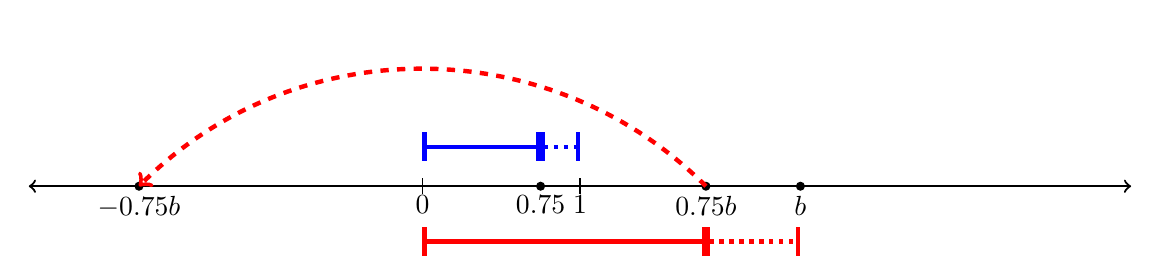
\begin{tikzpicture}
\draw[ultra thick,blue][|-|] (-2,.5) -- (-.5,.5);
\draw[ultra thick,dotted,blue][|-|] (-.5,.5) -- (0,.5);
\draw[ultra thick,red][|-|] (-2,-.7) -- (1.6,-.7);
\draw[ultra thick,dotted,red][|-|] (1.6,-.7) -- (2.8,-.7);
\draw[thick] [->] (0,0) -- (7,0);
\draw[thick] [<-] (-7,0) -- (0,0);
\node[align=center,below] at (-2,0){$0$};\draw (-2,-.1) -- (-2,.1);
\node[align=center,below] at (0,0){$1$};\draw (0,-.1) -- (0,.1);
\node[align=center,below] at (2.8,0){$b$};\draw[fill](2.8,0)circle[radius=.05];
\node[align=center,below] at (-.5,0){$0.75$};\draw[fill](-.5,0)circle[radius=.05];
\node[align=center,below] at (1.6,0){$0.75b$};\draw[fill](1.6,0)circle[radius=.05];
\node[align=center,below] at (-5.6,0){$-0.75b$};\draw[fill](-5.6,0)circle[radius=.05];
\draw[ultra thick,->,dashed,red] (1.6,0) to [out=135,in=45] (-5.6,0);
\end{tikzpicture}
\caption{Multiplying by a negative is multiplying by a positive, then flipping across zero.}
\label{fig:mult4}
\end{figure}    

\begin{question} Explain why the following statements are true using pictures and words to represent the numbers involved:
\begin{enumerate}
\item[a.] A positive number times a positive number is positive.
\item[b.] A positive number times a negative number is negative.
\item[c.] A negative number times a negative number is positive.
\item[d.] If $a$ is any number, multiplying $a$ by $-1$ is the same as $ -a$.
\end{enumerate}
\end{question}

\vfill

\pagebreak

\section{Division and Fractions}

\subsection{Division and Multiplication}
We begin with our basic intuitive metaphors for fractions:\\

\begin{center}
Fractions as Pieces of a Whole
\begin{tabular}{|p{2in} c p{1.5in}|}
\hline\hline \it{Positions and Sizes} & & \it{Numbers}\\
\hline Starting at $0$, the distance so that $b$ steps of that size will be $1$. & $\longrightarrow$ & $\frac{1}{b}$ \\&&\\
Starting at $0$, the distance so that $b$ steps of that size will be $a$.& $\longrightarrow$ & $\frac{a}{b}$ \\&&\\
\hline
\end{tabular}

\end{center}

The metaphors of this table assume $b$ is a positive integer so that we may use the idea of multiplication as repeated addition to reach a more formal understanding of division. 


\begin{tcolorbox}{\bf Key Concept - Multiplication and Division as Inverse Operations of One Another} 

Since taking $b$ steps of size $\frac{a}{b}$ reaches $a$, we have the following identity:
\[
b\cdot\frac{a}{b} = a.
\]
When $a$ and $b$ are not integers, we use this identity to \underline{define}\ \normalfont what $\frac{a}{b}$ is: \it{For any numbers $a$ and $b$, $\frac{a}{b}$ is the unique number such that when it is multiplied by $b$ results in $a$.\ }\normalfont In other words, \it{division by $b$ is the inverse operation of multiplying by $b$. Likewise, division is the inverse operation of multiplication.}\normalfont 
\end{tcolorbox}

\vspace{.2in}
\begin{figure}[h]
\centering
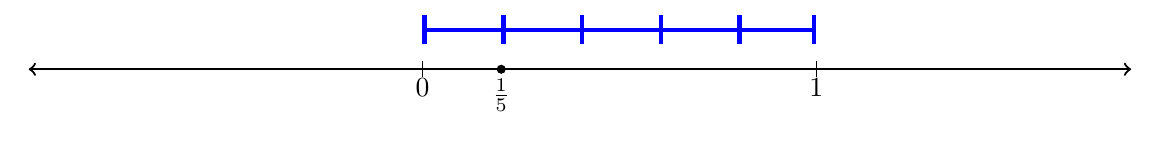
\begin{tikzpicture}
\draw[ultra thick,blue][|-] (-2,.5) -- (-1,.5);
\draw[ultra thick,blue][|-] (-1,.5) -- (0,.5);
\draw[ultra thick,blue][|-] (0,.5) -- (1,.5);
\draw[ultra thick,blue][|-] (1,.5) -- (2,.5);
\draw[ultra thick,blue][|-|] (2,.5) -- (3,.5);
\draw[thick] [->] (0,0) -- (7,0);
\draw[thick] [<-] (-7,0) -- (0,0);
\node[align=center,below] at (-2,0){$0$};\draw (-2,-.1) -- (-2,.1);
\node[align=center,below] at (3,0){$1$};\draw (3,-.1) -- (3,.1);
\node[align=center,below] at (-1,0){$\frac{1}{5}$};\draw[fill](-1,0)circle[radius=.05];
\end{tikzpicture}
\caption{$\frac{1}{5}$ is the size of a piece of $1$ when it is divided into $5$ pieces of equal size.}
\label{fig:div1}
\end{figure}   

\begin{question}
Explain why $\dfrac{a}{a} = 1$.
\end{question}

\begin{question}
What does $a \cdot \dfrac{1}{b}$ mean?  
\end{question}
\vfill

\begin{tcolorbox}{\bf Fundamental Fraction Properties:}

There are four fundamental properties that we must internalize about fraction in order to do arithmetic with them:
\begin{enumerate}
\item $\dfrac{a}{a} = 1$
\item $\dfrac{a}{1} = a$
\item $x\cdot\dfrac{a}{b} = \dfrac{xa}{b}$
\item $\dfrac{xa}{xb} = \dfrac{a}{b}$
\end{enumerate}
\tiny{(From \ttfamily http://gdaymath.com/lessons/fractions/2-5-the-key-fraction-property/\normalfont)}
\end{tcolorbox}

\par

\begin{question} \begin{enumerate}
    \item[a.] What do you get when you multiply $\dfrac{b}{a}$ by $\dfrac{a}{b}$?  
    \item[b.] What do you get when you multiply $\dfrac{1}{\left(\frac  ab \right)}$ by $\frac{a}{b}$?  
    \item[c.] Explain why $\dfrac{1}{\left(\frac{a}{b}\right)} = \dfrac{b}{a}$. \end{enumerate}
\end{question}

\par

\begin{question}(Multiplying Fractions) Explain why $\dfrac{a}{b}\cdot\dfrac{c}{d} = \dfrac{ac}{bd}$ using the fundamental fraction properties. 
\end{question}

\par

We can also use the stretch/squeeze metaphor of multiplication to give a geometric interpretation of $\frac{a}{b}$ when $b$ is not an integer. To do this, let's let $r = \frac{a}{b}$, and assume $a$ and $b$ are still positive (since negatives just reflect to the other side of zero). Our goal is to figure out where $r$ is on the number line. To do this, we first  do a manipulation:
\[
\frac{a}{b} = r \Longleftrightarrow a = rb.
\]
This manipulation  used the fact that multiplication by $b$ undoes division by $b$. From this manipulated equation we see that $r = \frac{a}{b}$ is the number that when stretched (if $b>1$) or squeezed (if $0<b<1$) by $b$ gives you $a$.


\begin{question} Explain the following two statements:
\begin{enumerate}
\item[a.] If $b$ is very large, then $\frac{1}{b}$ is very small.
\item[b.] If $b$ is very close to zero, but still positive, then $\frac{1}{b}$ is very large.
\end{enumerate} 
\end{question}

\par

Now let's consider why we must say $\frac{a}{0}$ is undefined no matter what $a$ is.
\begin{itemize}
\item {\bf Reason 1:} Consider the fraction $\frac{1}{b}$ where $b$ is positive. We know that if $b$ is very close to zero, then $\frac{1}{b}$ will be very large. For example, $\frac{1}{0.0001} = 10000$ because if you squeeze $10000$ by a factor of $0.0001$ you get $1$. However, you can always make the $b$ smaller and get a bigger number. This means that $\frac{1}{0}$ would need to be larger than every positive number. But no such number exists, so $\frac{1}{0}$ must be undefined.
\item {\bf Reason 2:} The expression $\frac{a}{0}$ should represent the number that when multiplied by $0$ results in $a$. However, any number multiplied by zero must be zero. For this reason, if $a$ is not zero, then $\frac{a}{0}\cdot 0$ cannot equal $a$. Thus we say that $\frac{a}{0}$ cannot represent a number if $a\neq 0$. 
\end{itemize}

\par
   To really see why the expression $\frac{0}{0}$ is undefined, you need an idea from Calculus, but you can get a feel for why it must be undefined in the next question.
\begin{question} Give a short reason why the expression $\frac{0}{0}$ could represent either $0$ or $1$. 
\end{question}

\subsection{Apples and Oranges: Units and Dimensional Analysis}
So far we have only talked about multiplying and dividing fractions. These operations with fractions are fundamentally easier then addition and subtraction. In order to build a useful metaphor of how to add and subtract fractions, it will be useful to talk about units of measurement. Not only will understanding units and unit conversion be useful for understanding fractions, but it is extremely useful in the sciences. 

\subsubsection{Dimensional Analysis and the Factor-Label Method of Unit Conversion} 
A very common task in physics or chemistry classes involves converting between units of measurement of quantities of the same dimension. The simplest way to do this is to treat the units of measurement as numbers multiplied by the numerical quantity in those units. So if we say a rod is two meters long, we would write the mathematical expression
\[
\mbox{length} = 2 \mbox{m},
\]
where $\mbox{m}$ is the abbreviation for meters multiplied by the number $2$. Since the unit name (the label) is multiplied by a number it is a factor in that expression. This is why we call this treatment of unit names as numbers the \it{factor-label method}\normalfont. By treating the units as number, we can use our prior knowledge of arithmetic operations to make conversions.
\par
\begin{eg} Suppose we need to convert $12$ ounces into milliliters. This is a legal conversion because both ounces and milliliters have the same dimension; both units describe volume. In order to make the conversion, we write down an equation with the number of one of the units in another:
\[
1 \mbox{oz} = 29.5735 \mbox{mL}.
\]
Form this equation, we can divide to obtain $1$ without units in two different ways:
\[
1=\frac{1 \mbox{oz}}{29.5735\mbox{mL}}\ \ \mbox{and} \ \ 1=\frac{29.5735 \mbox{mL}}{1 \mbox{oz}}.
\]
Multiplying the quantity $12 \mbox{oz}$ by either of these expressions for $1$ must leave it unchanged. In order to obtain final units of $\mbox{mL}$, we will multiply by the second because $\frac{\mbox{oz}}{\mbox{oz}} = 1$ (we say the units of ounces cancel).
\[
12\mbox{oz} = 12\mbox{oz}\cdot\frac{29.5735\mbox{mL}}{1\mbox{oz}} = 12\cdot 29.5735 \mbox{mL} = 354.882 \mbox{mL}.
\]
\qed
\end{eg}
\par

\begin{eg} A $rope$ is a unit of length equal to 20ft (it isn't used much anymore). Suppose an old city plan shows that the street is $2\ \mbox{rope}$ wide with a sidewalk that is $2$yd on each side. What is the total width of the street plus both sidewalks? You may be able to see quickly that the answer is 52ft,  but let's do all the conversions carefully.

\par 

First, note that we will need to add the width of both sidewalks to the width of the street. It isn't convenient to convert ropes to yards or yards to ropes; it makes the most sense to convert everything to feet. Let's write all our conversion equations:
\[
1 \mbox{street} = 2 \mbox{rope}\ ,\ 1\mbox{rope} = 20\mbox{ft}\ ,\ 1\mbox{sidewalk} = 2\mbox{yd}\ ,\ 1\mbox{yd} = 3\mbox{ft}.
\]
So we get the following:
\begin{eqnarray*}
1\mbox{street} + 2\mbox{sidewalk} & = & 1\mbox{street}\cdot\frac{2\mbox{rope}}{\mbox{street}}\cdot\frac{20\mbox{ft}}{\mbox{rope}} + 2\mbox{sidewalk}\cdot\frac{2\mbox{yd}}{\mbox{sidewalk}}\cdot\frac{3\mbox{ft}}{\mbox{yd}}\\\\
\ & = & 40\mbox{ft}+12\mbox{ft}= 52\mbox{ft}
\end{eqnarray*}\qed
\end{eg}
\par

\begin{question} Suppose a person is on a train that is moving $100$ km/hr and they run from the rear of the train to the front at a rate of $8$ m/s. How fast is this person moving relative to the ground in m/s? Note that $1$ km = $1000$ m and $1$ hr = $3600$ s.
\end{question}

\par

\begin{eg} The factor-label method of dimensional analysis can also be used to change the way we look at a changing quantity through multiplication and division. For instance, suppose a tank contains a salt water solution with a concentration of $2$ grams of salt per liter. If the tank is drained at a rate of $10$ mL/s, at what rate is salt leaving the tank in g/s?

\par

\underline{Solution:}\ \normalfont To solve this problem, let's first convert the draining rate into L/s: 
\[
10 \frac{\mbox{mL}}{\mbox{s}} = 10 \frac{\mbox{mL}}{\mbox{s}}\cdot \frac{1}{1000}\frac{\mbox{L}}{\mbox{mL}} = \frac{1}{100} \frac{\mbox{L}}{\mbox{s}}.
\]
Now we just need to multiply quantities to arrive at the correct units for the rate of salt leaving the tank:
\[
2\frac{\mbox{g}}{\mbox{L}}\cdot\frac{1}{100}\frac{\mbox{L}}{\mbox{s}} = \frac{2}{100}\frac{\mbox{g}}{\mbox{s}} = 0.02\frac{\mbox{g}}{\mbox{s}}
\]\qed
\end{eg}

\noindent{\bf Question 12:} The cost of fuel for a riverboat is $\$100$ per hour when moving $10$ miles per hour. In addition to fuel costs, the operating cost (paying the crew etc.) is $\$625$ per hour. What is the total cost in $\$$/mi when the boat is moving $10$ miles per hour?


\subsection{Adding and Subtracting Fractions}
Now that we have thought about real world units of measurement, and we can convert units that measure the same dimensional quantity, we can introduce a useful metaphor for adding, subtracting, and comparing fractions:
\begin{center}
Fractions as Units
\begin{tabular}{|p{2in} c p{1.5in}|}
\hline\hline \it{Units of Measurement} & & \it{Numbers}\\
\hline\ & \ & \\
Dimensional Unit of ``$b$-ths'' & $\rightarrow$ & $\frac{1}{b}$ \\&&\\
\hline
\end{tabular}  
\end{center}

Often it will be best to think of fractions as units of length (like when we think of numbers as positions on a line), but they could be areas, volumes, etc. Here we will think of the number $1$ as the basic unit of measurement. Then a $b$-th is the unit that goes into the basic unit $b$ times. For instance, if we are thinking of $1$ as $1$ foot, then $\frac{1}{12}$ is one inch because there are 12 inches in one foot.

\par

\begin{question} For each of the following basic units, what fraction does the given quantity represent? For instance, if the basic unit is one yard, then $1$ foot is $\frac{1}{3}$ because there are three feet in a yard.
\begin{enumerate}
\item[a.] Basic Unit: 1 kilometer. $100$ meters $ =$\underline{\hspace{1in}}. 
\item[b.] Basic Unit: 1 cup. $1$ ounce  $ =$\underline{\hspace{1in}}. 
\item[c.] Basic Unit: 1 meter. $10$ centimeters $ =$\underline{\hspace{1in}}. 
\item[d.] Basic Unit: 1 gallon. $3$ quarts $ =$\underline{\hspace{1in}}. 
\item[e.] Basic Unit: 1 football field. $40$ yards $ =$\underline{\hspace{1in}}.
\item[f.] Basic Unit: 1 tablespoon. $8$ teaspoons $ =$\underline{\hspace{1in}}.  
\end{enumerate}
\end{question}

Now let's revisit the example of ropes and yards from the last section. In order to add two ropes to four yards, it was necessary to convert both ropes and yards into a smaller unit that went into both ropes and yards evenly. Specifically, both were converted to feet to get a total of 52 feet. When we are just working with numbers we do something very similar; we find a common denominator.

\par

\begin{eg} Let's add $\frac{3}{5}$ to $\frac{1}{2}$. To get started we can look at it pictorially with $\frac{1}{3}$ and $\frac{1}{7}$ on number lines:
\vspace{.2in}
\begin{figure}[h]
\centering
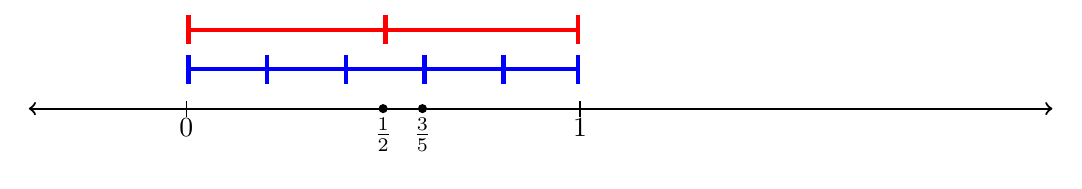
\begin{tikzpicture}
\draw[ultra thick,red][|-] (-5,1) -- (-2.5,1);
\draw[ultra thick,red][|-|] (-2.5,1) -- (0,1);
\draw[ultra thick,blue][|-] (-5,.5) -- (-4,.5);
\draw[ultra thick,blue][|-] (-4,.5) -- (-3,.5);
\draw[ultra thick,blue][|-] (-3,.5) -- (-2,.5);
\draw[ultra thick,blue][|-] (-2,.5) -- (-1,.5);
\draw[ultra thick,blue][|-|] (-1,.5) -- (0,.5);
\draw[thick] [->] (0,0) -- (6,0);
\draw[thick] [<-] (-7,0) -- (0,0);
\node[align=center,below] at (-5,0){$0$};\draw (-5,-.1) -- (-5,.1);
\node[align=center,below] at (0,0){$1$};\draw (0,-.1) -- (0,.1);
\node[align=center,below] at (-2,0){$\frac{3}{5}$};\draw[fill](-2,0)circle[radius=.05];
\node[align=center,below] at (-2.5,0){$\frac{1}{2}$};\draw[fill](-2.5,0)circle[radius=.05];
\end{tikzpicture}
\label{fig:addfracs1}
\end{figure} 

If we divide $\frac{1}{5}$ in half and $\frac{1}{2}$ into five pieces, we find that $\frac{1}{10}$ goes into both $\frac{1}{5}$ and $\frac{1}{2}$ evenly.

\vspace{.2in}
\begin{figure}[h]
\centering
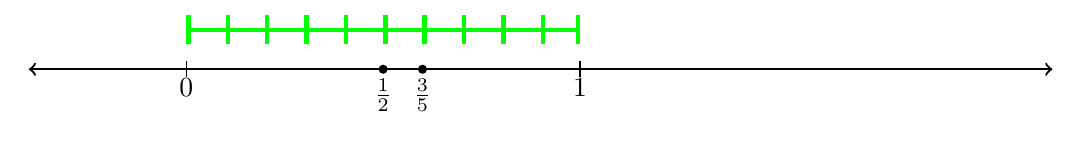
\begin{tikzpicture}
\draw[ultra thick,green][|-] (-5,.5) -- (-4.5,.5);
\draw[ultra thick,green][|-] (-4.5,.5) -- (-4,.5);
\draw[ultra thick,green][|-] (-4,.5) -- (-3.5,.5);
\draw[ultra thick,green][|-] (-3.5,.5) -- (-3,.5);
\draw[ultra thick,green][|-] (-3,.5) -- (-2.5,.5);
\draw[ultra thick,green][|-] (-2.5,.5) -- (-2,.5);
\draw[ultra thick,green][|-] (-2,.5) -- (-1.5,.5);
\draw[ultra thick,green][|-] (-1.5,.5) -- (-1,.5);
\draw[ultra thick,green][|-] (-1,.5) -- (-.5,.5);
\draw[ultra thick,green][|-|] (-.5,.5) -- (0,.5);

\draw[thick] [->] (0,0) -- (6,0);
\draw[thick] [<-] (-7,0) -- (0,0);
\node[align=center,below] at (-5,0){$0$};\draw (-5,-.1) -- (-5,.1);
\node[align=center,below] at (0,0){$1$};\draw (0,-.1) -- (0,.1);
\node[align=center,below] at (-2,0){$\frac{3}{5}$};\draw[fill](-2,0)circle[radius=.05];
\node[align=center,below] at (-2.5,0){$\frac{1}{2}$};\draw[fill](-2.5,0)circle[radius=.05];
\end{tikzpicture}
\label{fig:addfracs2}
\end{figure} 

Now we see the addition:
\[
\frac{3}{5} + \frac{1}{2} = \frac{6}{10}+\frac{5}{10} = \frac{11}{10}.
\]
This is the geometric way of visualizing the process known as  known as ``cross multiplying''. That is when you multiply each part of a fraction with a fraction equal to one in order to have a common denominator:
\[
\frac{3}{5}+\frac{1}{2} = \frac{2}{2}\cdot\frac{3}{5} + \frac{5}{5}\cdot\frac{1}{2} = \frac{11}{10}.
\]\qed
\end{eg}

\par

One thing we usually try to find is the \underline{least} common denominator between two fractions. Thinking in terms of units, this is like finding the largest possible unit that goes into both quantities evenly. In the example given above we could have used $\frac{1}{20}$ to go into $\frac{1}{2}$ and $\frac{3}{5}$ evenly and obtained
\[
\frac{3}{5}+\frac{1}{2} = \frac{22}{20}.
\]
However, that makes the numbers we are dealing with larger for no reason. This would be like converting both ropes and yards into inches; it's possible, but unnecessary.
  
\par     
 \begin{question}
 Draw  a picture to carefully perform the following:
 \begin{enumerate}
     \item[a.] $\frac12 + \frac13$
     \item[b.] $\frac12+\frac14$
     \item[c.]  $\frac13+\frac14$
 \end{enumerate}
 \end{question}
\begin{question} Perform the indicated additions and subtractions:
\begin{enumerate}
\item[a.] $\frac{3}{7}+\frac{9}{8}$
\item[b.] $\frac{7}{3}+\frac{8}{9}$
\item[c.] $\frac{1}{2} + \frac{1}{3} - \frac{1}{4}$
\item[d.] $\frac{15}{3}  + \frac{14}{7}$
\end{enumerate}
\end{question}

\section{Exponents}
Most fundamentally, exponents represent repeated multiplication in the way that multiplication represents repeated addition. 

\begin{center}
Multiplication is to Addition as Exponents are to Multiplication
\begin{tabular}{|p{2.5in} c p{2.5in} |}
\hline\hline \it{Multiplication as Repeated Addition} & &\it{Exponents as Repeated Multiplication}\\
\hline $na = \underbrace{a+ a +\cdots + a}_\text{$n$ times}$ & $\longrightarrow$ &  $a^n = \underbrace{a\cdot a \cdot\cdots \cdot a}_\text{$n$ times}$\\
\hline
\end{tabular}
\end{center}

Based on this idea, we can see the following properties of exponents:
\begin{tcolorbox}
{\bf Properties of Exponents}
\begin{itemize}
\item $a^na^m = a^{n+m}$. \phantom{wwww} Eg $2^{3}\cdot 2^4 = 2\cdot 2\cdot 2\cdot 2\cdot 2\cdot 2\cdot 2 = 2^7 = 128$.
\item If $a\neq 0$, $\frac{a^n}{a^m} = a^{n-m}$. 
 \phantom{www} Eg  $\frac{3^{5}}{3^2} = \frac{3\cdot 3\cdot 3\cdot 3\cdot 3}{3\cdot 3} = 3^3 = 27$.
\item $(a^n)^m = a^{nm}$. 
 \phantom{wwww} Eg  $(2^{3})^2 = (2\cdot 2\cdot 2)\cdot(2\cdot 2\cdot 2) = 2^6 = 64$.
\item $(ab)^n = a^nb^n$. 
 \phantom{www} Eg  $(2\cdot 3)^2 = (2\cdot 3)\cdot (2\cdot 3) = 2\cdot 2\cdot 3\cdot 3 $ \phantom{wwwwwwwwwwwwww} $ = 2^2\cdot3^2 = 36$.
\item $\left(\frac{a}{b}\right)^{n} = \frac{a^n}{b^n}$. 
 \phantom{wwwww} Eg  $\left(\frac{2}{3}\right)^2 = \frac{2}{3}\cdot\frac{2}{3} = \frac{4}{9}$.
\end{itemize}
\end{tcolorbox}

More subtlety arises when making sense out of zero, negative, and fractional exponents. The problem is that we don't know what it means to multiply a number by itself zero times, a negative number of times, or a fractional number of times. Because of this, we  use the properties listed above to define zero, negative, and fractional exponents.
\par
First, let's consider what $a^0$ should equal, where $a$ is a nonzero number. We know that if $n$ is any number that $0 = n-n$. Using the second exponent property given above, we have
\[
a^0 = a^{n-n} = \frac{a^n}{a^n}.
\]
Since $\frac{a^n}{a^n} = 1$, we define $a^0 = 1$ whenever $a$ is not zero ($0^0$ is undefined).
\par 
Now consider a negative exponent, $a^{-n}$. Here we use the first two exponent properties to arrive at what $a^{-n}$ must be. We have
\[
a^{n}a^{-n} = a^{n+(-n)} = a^{n-n} = a^{0} = 1.
\]
Shortening this string of equalities, we have $a^{n}a^{-n} = 1$. Now we divide both sides by $a^{n}$ to get $a^{-n} = \frac{1}{a^{n}}$. In words, a negative exponent denotes division by the same number with a positive exponent.

\par
 
Finally, let's consider what $a^{\frac{1}{n}}$ should be. This time we'll use the third exponent property that a power raised to a power reults in the exponents being multiplied. Thus we have,
\[
(a^{\frac{1}{n}})^n  = a^{\frac{n}{n}} = a^{1} = a.
\]
So $a^{\frac{1}{n}}$ is the number that when raised to the $n$-th power results in $a$. This is exactly a description of the $n$-th root, $\sqrt[n]{a}$. Going slightly further with the third exponent property, we have $a^\frac{m}{n} = \sqrt[n]{a^m} = (\sqrt[n]{a})^m$.
\par 
\begin{question} Justify the last sentence of the last paragraph.
\end{question}
\par 
So in summary we have:
\begin{tcolorbox}
{\bf Zero, Negative, and Fractional Exponents}
\begin{itemize}
\item $a^0 = 1$ when $a\neq 0$.
\item $a^{-n} = \frac{1}{a^n}$:  \phantom{w}   negative exponents denote division.
\item $a^{\frac{m}{n}} =  \sqrt[n]{a^m} = (\sqrt[n]{a})^m$:  \phantom{w} denominators in fractional exponents \phantom{wwwwwwwwwwwwwww} denote roots.
\end{itemize}
\end{tcolorbox} 


\par

\begin{question} Evaluate the following without a calculator. Make sure you do it as efficiently as possible using properties of exponents.
\begin{enumerate}
\item[a.] $4^{\frac{3}{2}}$
\item[b.] $9^{-\frac{1}{2}}$
\item[c.] $(\frac{1}{27})^{-\frac{2}{3}}$
\item[d.] $\frac{1}{7^{-2}}$
\item[e.] $\frac{10^9}{10^7}$
\item[f.] $16^{\frac{5}{4}}$
\end{enumerate}
\end{question}

\begin{question} Use properties of exponents to write the following in a simpler way using only positive exponents.
\begin{enumerate}
\item[a.] $ -4^0$
\item[b.] $ z^{-3} \cdot z^3$
\item[c.] $ w^{-4} \cdot(4x)^0 \cdot x^6$
\item[d.] $  \dfrac{5t^3}{t^{-6}}  $
\item[e.] $ \left(\dfrac{a^2}{b^3} \right)^{-1} $
\item[f.] $ \left(\dfrac{x}{3} \right)^{-2} $
\end{enumerate}
\end{question}

\section{Parentheses and Order of Operations}

Each of the previous sections in this chapter have focused mostly on one mathematical operation at a time. However, it is often the case that more than one operation is performed. Difficulty arises because the order in which operations occur matters; different orders yield different results. For example, let's consider the two mathematical processes described below:
\begin{enumerate}
\item Take the number two, add three to it, then multiply the result by four.
\item Take the number two, multiply it by four, then add three to the result.
\end{enumerate}
The two operations are adding three and multiplying by four, but performed in different orders. In the first order, two gets shifted up to five, then stretched out by a factor of four, yielding an end result of 20. In the second, two gets stretched out to eight, then that is shifted up by three, yielding an end result of 11. In order to distinguish these two orders using mathematical notation, we use parentheses to enclose those procedures that are to be performed first. Specifically, we have the following symbolic representations corresponding to the verbal descriptions given above:
\begin{enumerate}
\item $4(2+3) = 20$
\item $(4\cdot 2)+3 = 11$
\end{enumerate}
In a mathematical expression, any procedures that are enclosed in parentheses are meant to be performed before those procedures outside that set of parentheses. One way to think of parentheses is that whatever is inside them must be combined/simplified to a single quantity before proceeding. 
\par
What about the other operations? You probably have learned the answer earlier in your mathematical lives. Indeed, in the last section we used parentheses in expressions with exponents without really explaining their use. You may have even encountered some mnemonic device for remembering order of operations. Because being able to execute the operations is more important than just remembering, we will catalog the order of operations rules here, then use them in some problems.

\vfill
\pagebreak

\begin{tcolorbox}
{\bf Order of Operations}
\begin{itemize}
\item Procedures enclosed in parentheses should be performed before any operations outside those parentheses.
\item Exponents should be applied second, but only to the object that the exponent is directly above and to the right of.
\item Multiplication and/or division should be performed before addition and/or subtraction unless otherwise indicated by parentheses. In other words, in an expression only involving addition and multiplication, those individual multiplications are in parentheses.
\item Division is just multiplication by the reciprocal, so division and multiplication can be performed in either order.
\item Subtraction is just addition of a negative, so subtraction and addition can be performed in either order.
\end{itemize}
\end{tcolorbox}

These aren't actually too hard to keep track of, just as long as you remember that their purpose is to remove ambiguity from mathematical notation. For instance, without these rules $4\cdot 2 +3$ could be interpreted either as $11$ or $20$. These rules make sure that we all agree that it is $11$. 
\par 
In addition to multiplications having understood (but not written down) parentheses around them, there are often understood parentheses in fractions. For instance, if we write
\[
\frac{1}{3+7},
\]  
we will understand that $3+7$ is to be performed first. Usually this isn't an issue when fractions are written with horizontal lines, but we would have to use parentheses to write it on a single line as $1/(3+7)$.

\begin{question} Evaluate each of the following quantities without a calculator. If your answer is a fraction, give it in reduced form.
\begin{enumerate}
\item[a.] $3\cdot 3^{-2}\cdot(-1)^2$
\item[b.] $-3^2+\frac{64}{2^3}$
\item[c.] $(-5+2)^3+12$
\item[d.] $\frac{(3+2)^2}{4} - \left(\frac{2-7}{2}\right)^2$
\item[e.] $4+5/7$
\item[f.] $(4+5)/7$
\end{enumerate}
\end{question}

\begin{question} Verbally describe the sequence of operations performed on the number $a$ in the correct order.
\begin{enumerate}
\item[a.] $2(a+1)$
\item[b.] $2a+1$
\item[c.] $1-3\left(\frac{a}{2}+4\right)$
\item[d.] $3-2(a+5)$
\end{enumerate}
\end{question}

Now we come to the end of our chapter on arithmetic with numbers. Those of you with some exposure to algebra may now say, ``This is easy, but algebra is very different and difficult.'' The truth is that is we keep the representations of arithmetic operations from this chapter in mind, algebra will not be that difficult.
